\section{Theoretical Analysis}

In this section, we will perform a theoretical analysis that determined the behavior of the Recycling Folded Cascode (RFC) Operational Transconductance Amplifier (OTA) circuit. The main goal of this analysis is to understand the behavior of the circuit and to determine the values of the different parameters that will allow us to achieve the desired performance.

\textcolor{red}{explicar os main blocos do circuito}

\begin{figure}[H]
    \centering
    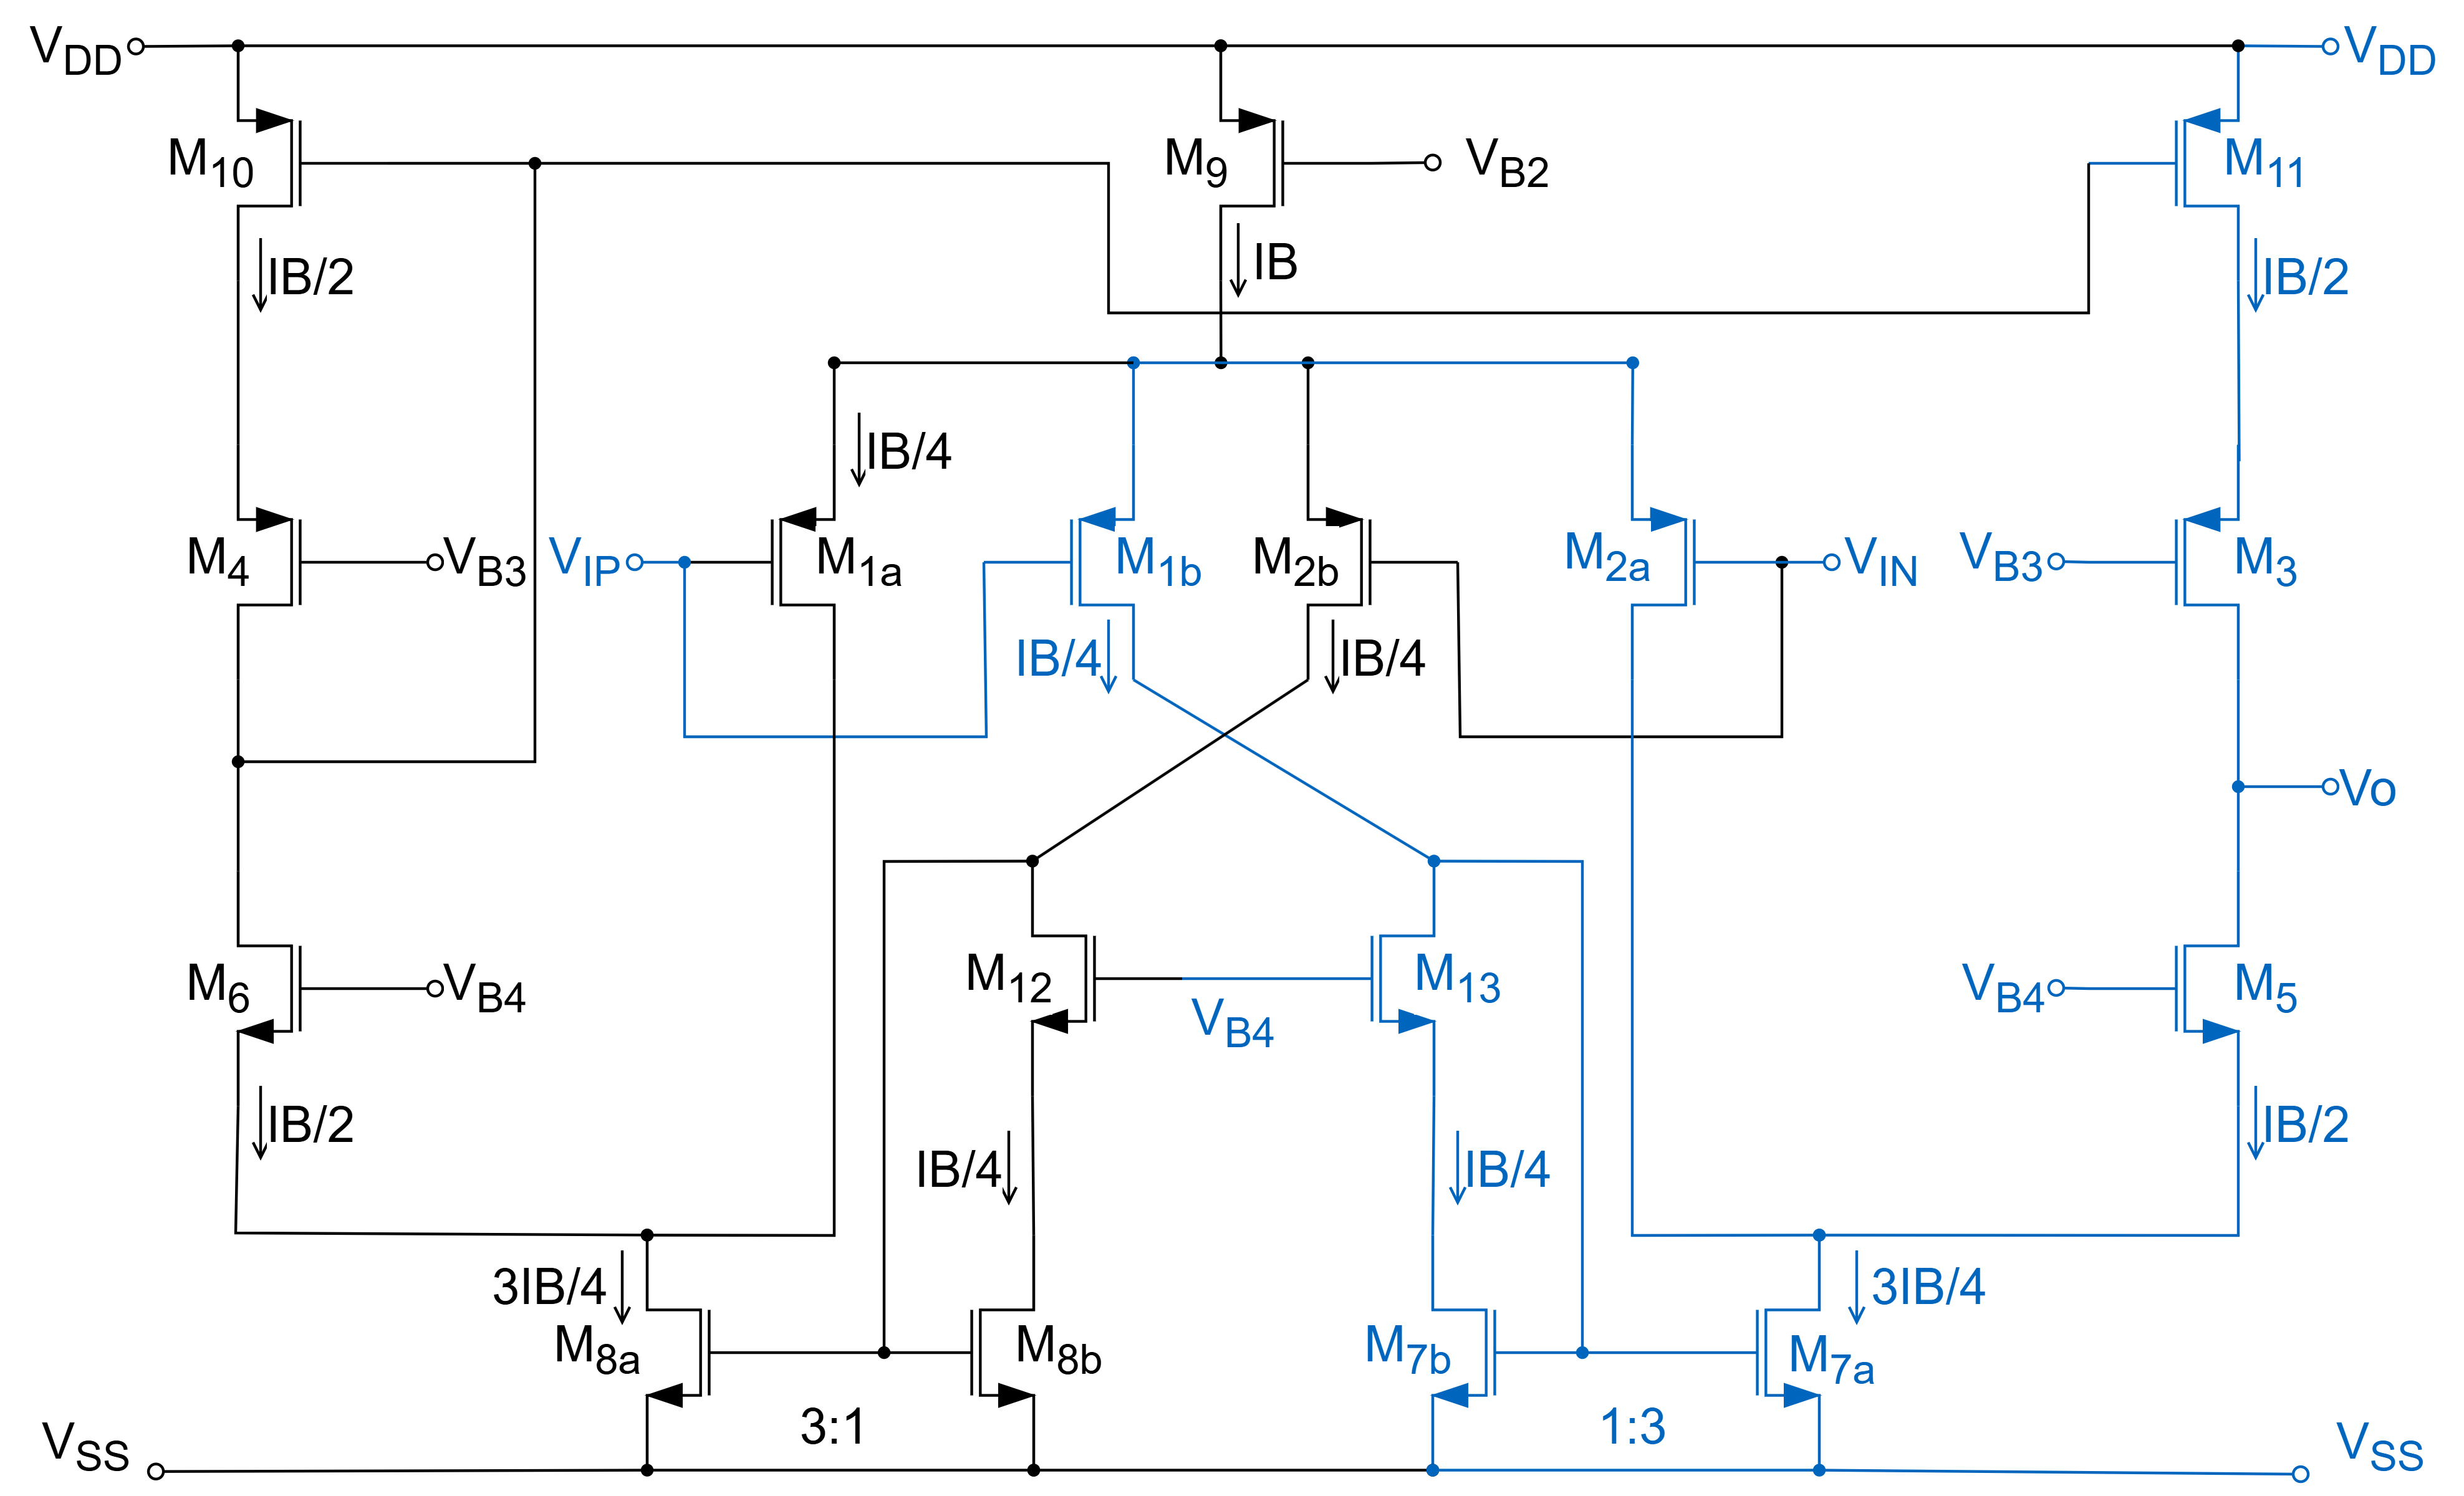
\includegraphics[width=1\textwidth]{Images/full_sch.png}
    \caption{Full Schematic without biasing circuit}
    \label{fig:full_schematic}
\end{figure}

\begin{figure}[H]
    \centering
    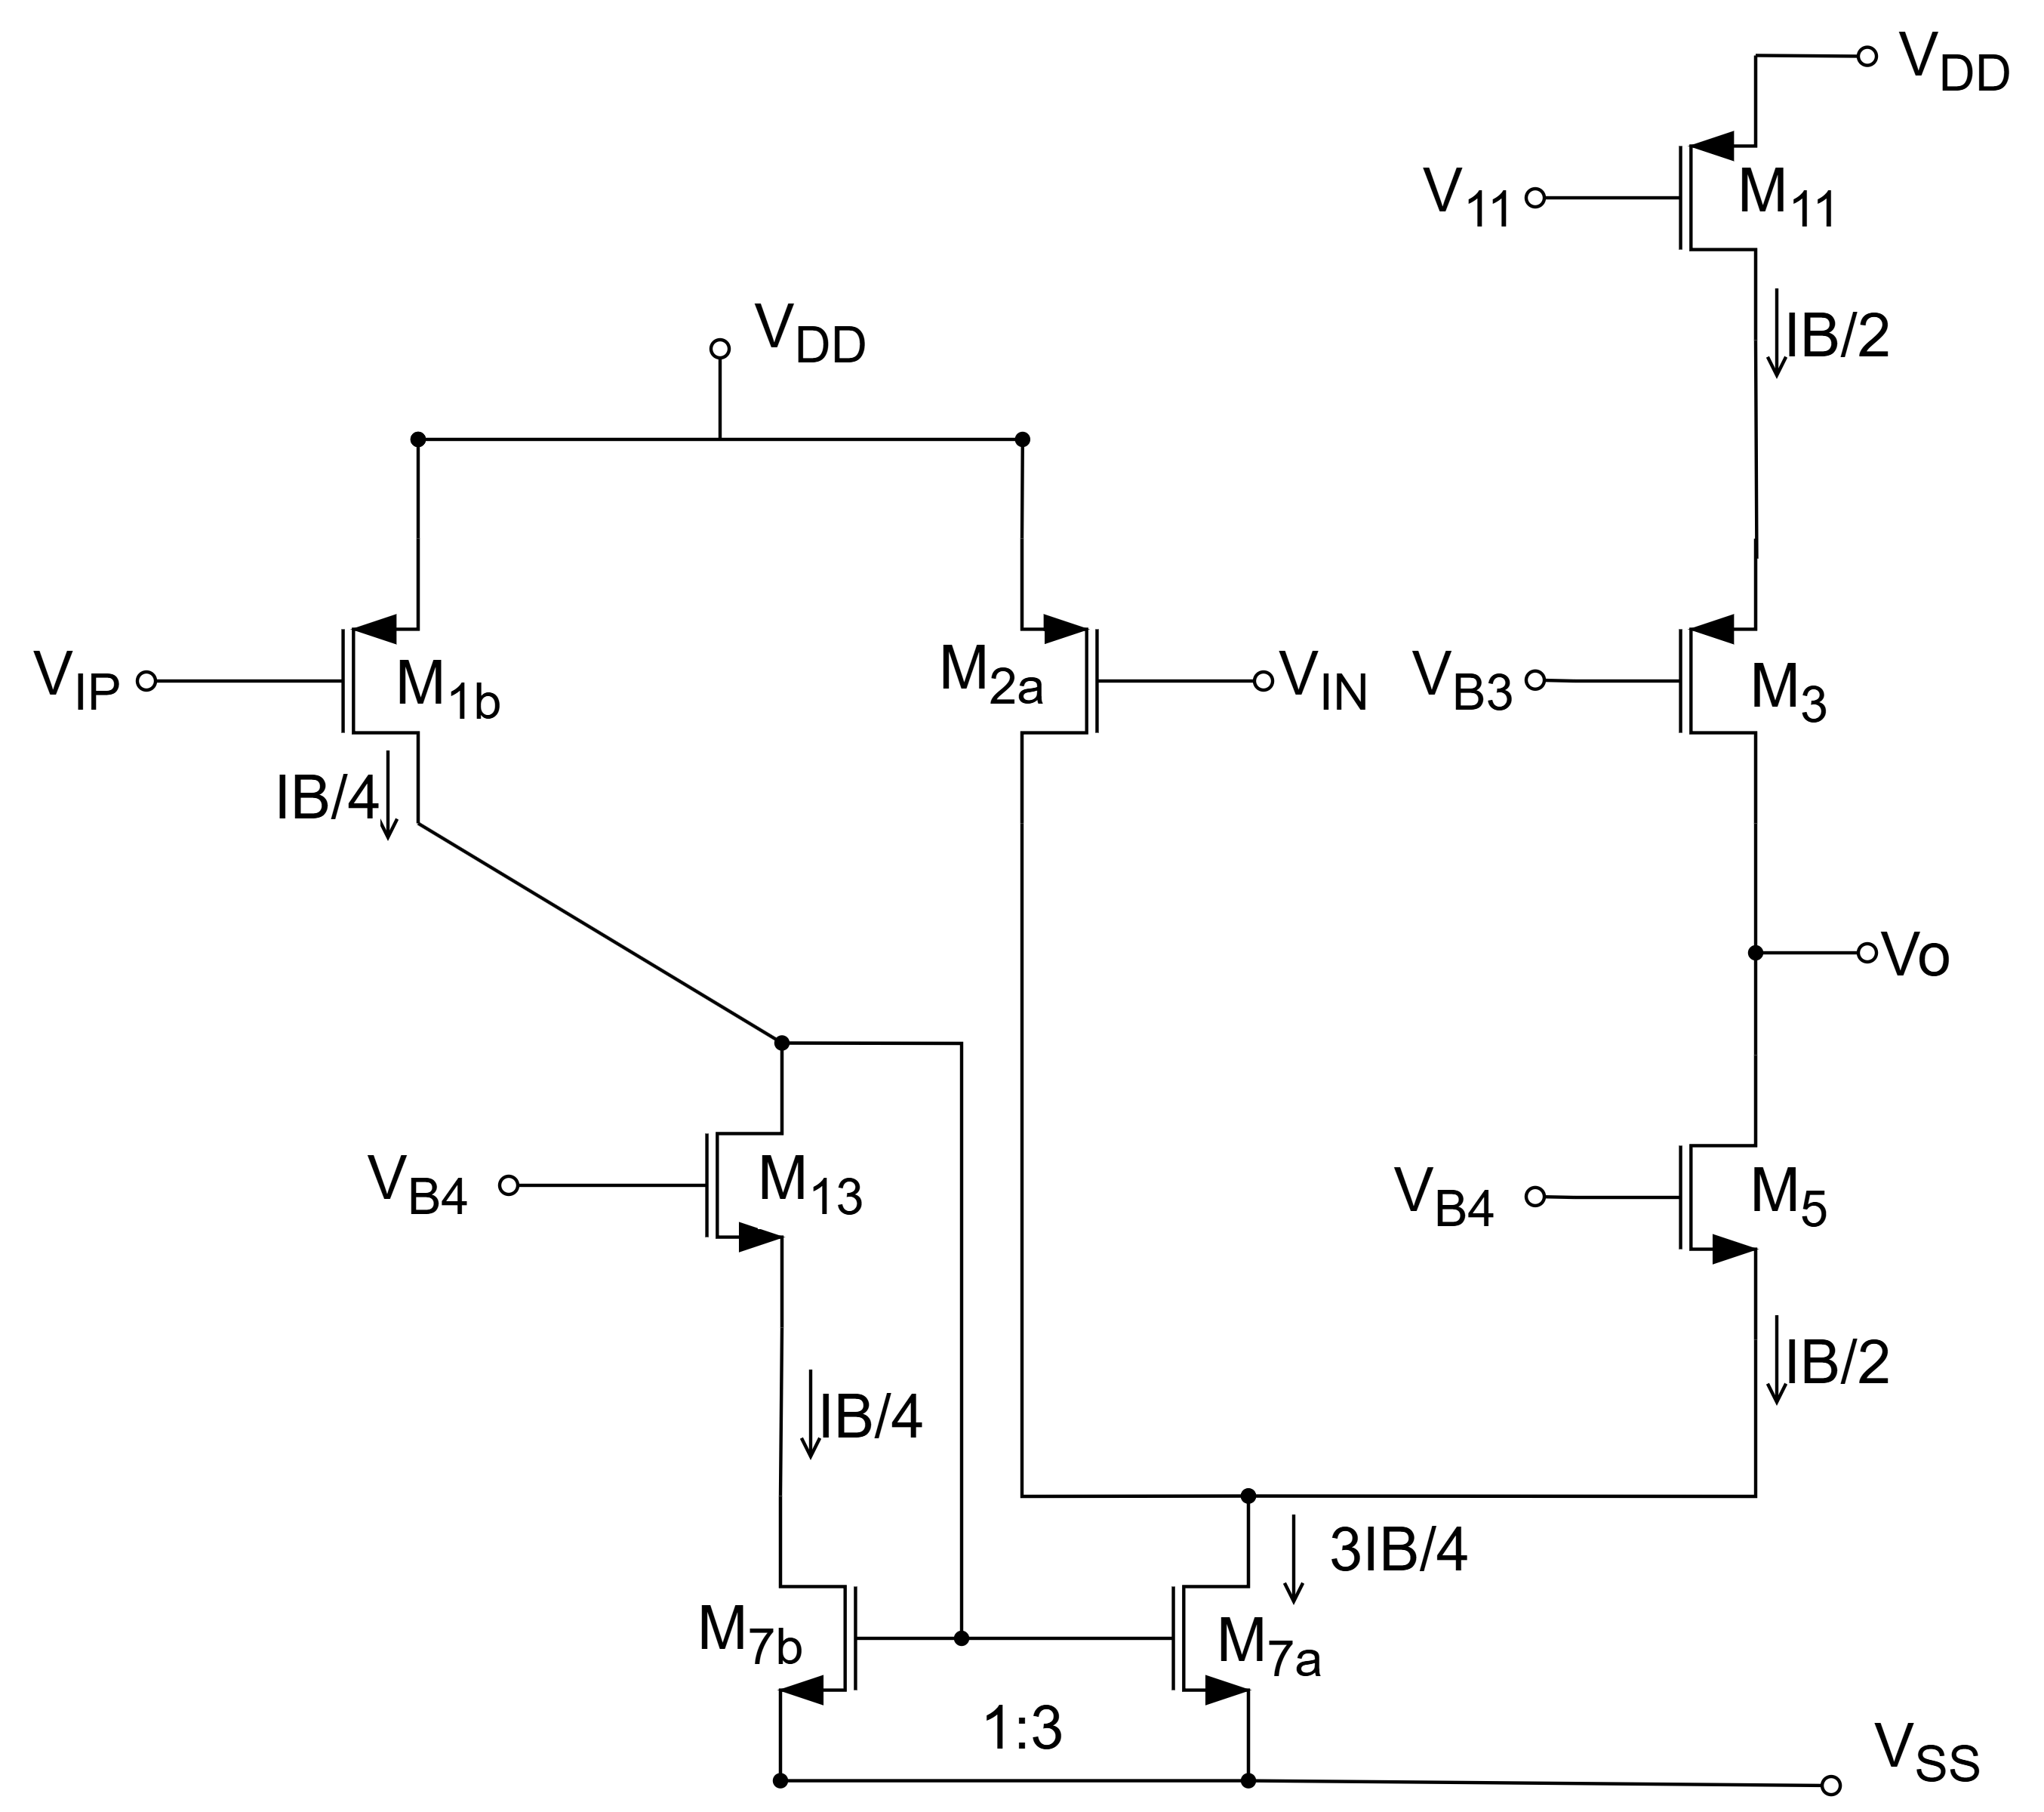
\includegraphics[width=0.6\textwidth]{Images/simplified_sch.png}
    \caption{Simplified Schematic}
    \label{fig:simplified_schematic}
\end{figure}



\textcolor{red}{explicar como chagamos ás expressoes por esquematico de parte do circuito que analizamos}
\subsection {DC Gain}

The DC gain of the circuit is given by $A_v$ where $G_M$ is the total transcondutance responsible for the gain of the circuit and $g_{out}$ is the conductance (inverse of the resistance) Seen from the output of the circuit.

$$A_v =  \frac{G_M}{g_{out}} \geq 66\hspace{0.1cm}dB$$

Where:
\begin{equation}
    \begin{cases}
        G_M = g_{m2a} + g_{m1b} \cdot \frac{g_{m7a}}{g_{m7b}} \approx g_{m2a} + 3 \cdot g_{m1b} \\
        g_{out} = g_{op} + g_{on}
    \end{cases}
\end{equation}

The total conductance seen from the output can be broken into 2 parts, conductance \textit{up} $g_{op}$ seen from the output node to the upper part of the circuit $V_{dd}$ and conductance \textit{down} $g_{on}$ seen from the output node to the lowest part of the circuit $V_{ss}$.

\begin{equation}
    \begin{cases}
        g_{op} = g_{ds11} \cdot \frac{g_{ds3}}{g_{m3}} \\
        g_{on} = \left( g_{ds2a} + g_{ds7a} \right) \cdot \frac{g_{ds5}}{g_{m5}}
    \end{cases}
\end{equation}

\subsection{Gain Bandwidth Product (GBW)}
The gain bandwidth product can be obtained by the ratio between $G_M$ and $C{out}$ where $C{out}$ is the equivalent capacitance seen from the output node.

$$  GBW = \frac{G_M}{C_{out}} >= 100 MHz $$

$C_{out}$ is given by :

$$C_{out} = C_L + C_{bd3} + C_{gd3} + C_{bd5} + C_{gd5}$$

\newpage

\textcolor{red}{ver qual é fp2 e fp3 - fpx ou fpz }

\subsection{Pole Frequencies}
in order to guarantee \textbf{stability in a unity-gain closed-loop} Configuration we need to define the frequencies
for poles $f_{px}$ and  $f_{pz}$

$$f_{px} = \frac{1}{C_x\cdot r_x} > x  \hspace{2cm}  f_{pz} = \frac{1}{C_z\cdot r_z} > y$$

Thus, we will need to calculate the equivalent capacitance and resistance at node $x$ and $y$ given by:

\begin{equation}
    \begin{cases}
        C_x = C_{gd7a} + C_{bd7a}+ C_{gd2a} + C_{bd2a} + C_{gd5} + C_{bs5}\\
        C_z = C_{gs13} + C_{bs13} + C_{bd7b}+ C_{gs7b} \\
        r_z \approx \frac{1}{gm13} \\
        r_x \approx g_{m5} 
    \end{cases}
\end{equation}

\subsection{Output Swing}
The output swing of the amplifier can be obtained by the following expression following a margin $V_{margin}$ of 80 mV or 0.08 V :

$$OS = V_{DD} - V_{DSsat11} - V_{DSsat3} - V_{DSsat5} - V_{DSsat7a} - 0.08  \geq  0.5 \hspace{0.2cm} V_{p-p}$$

\subsection{Excess-Noise Factor}
The Excess-Noise factor is the additional noise created by an amplifier with gain $A_v$. An amplifier with excess noise of 1 means that the intrinsic noise is multiplied by 1 therefore, the noise is not made any worse, but any value over 1 means the noise is increased due to the gain, we can calculate the value for Excess-Noise factor $\Gamma$ given by the following equation:

$$\Gamma = 1 + \frac{3}{4}\cdot \frac{gm_{8a}}{gm_{1a}} + \frac{1}{4}\cdot \frac{gm_{10}}{gm_{1a}}$$

\subsection{Power Dissipation}

Its intended that the power dissipation $P_D$ is minimized in order to have the best performing low power amp.

Where: 

$$P_D = V_{DD} \times \left(2 \times I_B + \dfrac{I_B\cdot 4}{10}\right) $$

\subsection{Figure of Merit (FoM)}
 We will also need to achieve the best possible figure-of-merit FoM defined by: 

$$FoM = 1000 \times \dfrac{GBW \times C_L}{P_D}$$
